\documentclass[11pt,a4paper]{article}
\usepackage[margin=2cm]{geometry}
\usepackage{cite,amsmath,amssymb,graphicx,booktabs,url,xcolor,titlesec,float}
\renewcommand{\familydefault}{\sfdefault}
\definecolor{acc}{RGB}{29,92,138}
\titleformat{\section}{\Large\bfseries\color{acc}}{\thesection.}{0.5em}{}
\titleformat{\subsection}{\large\bfseries\color{acc}}{\thesubsection}{0.5em}{}
\usepackage{caption}\setlength{\parskip}{0.5em}\setlength{\parindent}{0pt}\captionsetup{font=small}

\title{\bfseries\color{acc} Predicting a Water Quality Index Without Data Leakage\\[2pt]\large\mdseries\color{black}A study using classical machine learning}
\author{Priyal, Anusha, Sarthak, Kashika and Vaishnavi\\Newton School of Technology\\Advanced Machine Learning / Deep Learning, Project 18}
\date{}
\begin{document}\maketitle
\begin{abstract}\noindent
A water quality index turns many water measurements into one score between 0 and 100. In this project we train models to predict this score (the CCME index) from a small set of readings, and we compare four models: a baseline that always guesses the average, Ridge Regression, Random Forest and XGBoost. The index is calculated from eight measurements, so giving all eight to a model lets it simply work out the formula (R$^2$ = 0.991), which proves nothing. We therefore hide five of these measurements from the models. We test on monitoring stations the models have never seen, and separately on later years. On the unseen stations, XGBoost was best with MAE 7.543, RMSE 11.058 and R$^2$ = 0.293, slightly ahead of Random Forest (R$^2$ = 0.278). On later years, XGBoost reached R$^2$ = 0.243. The models predict polluted water to be better than it is, and much of their skill comes from knowing the country and the past readings of a station. Overall, tree models work better than a straight-line model, but a lot of the variation in the score is still unexplained.
\end{abstract}
\noindent\textbf{Keywords:} water quality index, regression, Random Forest, XGBoost, data leakage, SHAP.

\section{Introduction}
Authorities test rivers, lakes and coastal water to protect people and nature. A water quality index combines many measurements into one number, which is easier to report and compare. If a model could predict this number from a few simple readings, it could help with screening. But a high score from a model is only meaningful if the test is fair. In particular, if the model is given the same measurements that the index is calculated from, it can just recompute the formula instead of really predicting anything.

In this project we predict \texttt{target\_ccme\_value}, a CCME water quality index between 0 and 100 (higher means cleaner water). Our main contributions are: (1) an experiment that shows how much the formula leaks when all measurements are given, and a smaller input set that avoids it, (2) a fair test on stations the models have never seen, plus a second test on later years, and (3) a comparison of four models using MAE, RMSE and R$^2$, with confidence intervals and a look at where the models go wrong. The report first reviews related work, then describes the data and methods, and finally reports the results, limitations and our plan for Phase 2.

\section{Related Work}
The CCME index is based on how many measurements break their guideline, how often, and by how much \cite{ccme2001}. Reviews of surface-water quality describe the many water quality indices and pollution indices in use \cite{syeed2023}. They also point out weaknesses: one very bad measurement can be hidden by good ones, information about how measurements interact is lost, and the choice of measurements is partly subjective \cite{chidiac2023}. Karim et al.\ released a large dataset of surface-water measurements from 1940 to 2023 \cite{karim2025}. We use only a cleaned part of it, so our counts are different from the original dataset.

Random Forests use many decision trees built on random parts of the data \cite{breiman2001}. Gradient boosting builds a model step by step, where each step fixes the mistakes of the earlier ones \cite{friedman2001}, and XGBoost is a fast and well-controlled version of this idea \cite{chen2016}. SHAP is a method that shows how much each input pushed a prediction up or down \cite{lundberg2017}; it shows what the model uses, not what actually causes pollution. Other studies found that deep neural networks do not always beat tree models on table-like data \cite{grinsztajn2022,shwartz2022}.

Water quality studies use different tasks and measures, so their results are hard to compare. Ooko et al.\ found that Random Forest worked best, with 79\% accuracy, in a water quality classification study \cite{ooko2023}. Rahman et al.\ reported 97.33\% accuracy for sorting samples into five CCME classes on the Canadian part of the same dataset, using the eight measurements as inputs \cite{rahman2026}. Since the index is calculated from those eight measurements, such scores cannot be compared with ours. Section~\ref{sec:leak} shows that giving a model all eight measurements gives R$^2$ = 0.991.

The gap we focus on is the way models are tested. Scores can look better than they really are when the model is given the measurements the target is made from, or when the same station appears in both training and test data. We hide five of the main measurements, test on stations the model has not seen, add a test on later years, and use the same measures for every model. We do not claim that earlier studies all made these mistakes.

\section{Dataset and Exploratory Data Analysis}\label{sec:eda}
\subsection{Overview}
After cleaning, our dataset has 259,774 rows from 9,940 monitoring stations in England, Ireland, the USA and Canada, from 2000 to 2023. Each row is one water sample taken at one station on one date. The target \texttt{target\_ccme\_value} is the CCME score, a number from 0 to 100 where a higher score means cleaner water. The original dataset has 2.82 million records from five countries \cite{karim2025}; we keep a part of it that suits our fair-testing plan. The data are very uneven between countries: England has 69.3\% of the rows, Ireland 27.1\%, the USA 2.6\% and Canada 1.0\%. Because of this we report results for each country and not only one overall score.

\subsection{Problems we found in the raw data}
We looked at the raw data before using it and found five problems (Table~\ref{tab:clean}). First, many samples are effluent, sewage or drainage water. This is water from pipes and treatment works, not rivers, lakes or coasts, so we removed it. Second, we removed records before 2000, because the early years are thin and uneven. Third, we removed exact duplicate rows and impossible values (for example a pH above 14 or a temperature above 40\,$^\circ$C).

The fourth problem was the most surprising. The authors of the source data had filled many gaps with one repeated number for each country and water type, for example dissolved oxygen 10.2 in 360,401 English rows. Real measurements do not repeat like this: in a histogram they show up as one very tall thin spike. We found these values by how often they appeared and marked them as missing. They may still affect the score, because the index was calculated after the gaps were filled. Fifth, we removed rows with fewer than 5 real measurements out of 8, and we kept whole stations when reducing the size of the dataset, so that each station keeps its full history.
\begin{table}[H]\centering\small\caption{Main cleaning steps (counts from the cleaning log)}\label{tab:clean}
\begin{tabular}{p{4.3in}r}\toprule Step & Rows\\\midrule
Effluent, sewage, drainage removed & 635,532\\
Records before 2000 removed & 243,089\\
Exact duplicates removed & 7,277\\
Rows with fewer than 5 of 8 real measurements removed & 474,227\\
Final dataset after keeping whole stations & 259,774\\\bottomrule\end{tabular}\end{table}

\subsection{Missing values}
A missing value does not always mean a filler number that we removed. It can also mean that the measurement was never taken at that place (Figure~\ref{fig:miss}). For example, BOD is missing in all USA rows, nitrogen in 76.5\% of Canadian rows and pH in 69.5\% of USA rows. Over all rows, BOD is missing in 51.7\%, ammonia in 29.4\% and nitrate in 23.8\%, while temperature (0.6\%) and pH (4.5\%) are almost always there. Because of this, the models fill the gaps using the training data only, and they also get a flag that says a value was missing.
\begin{figure}[H]\centering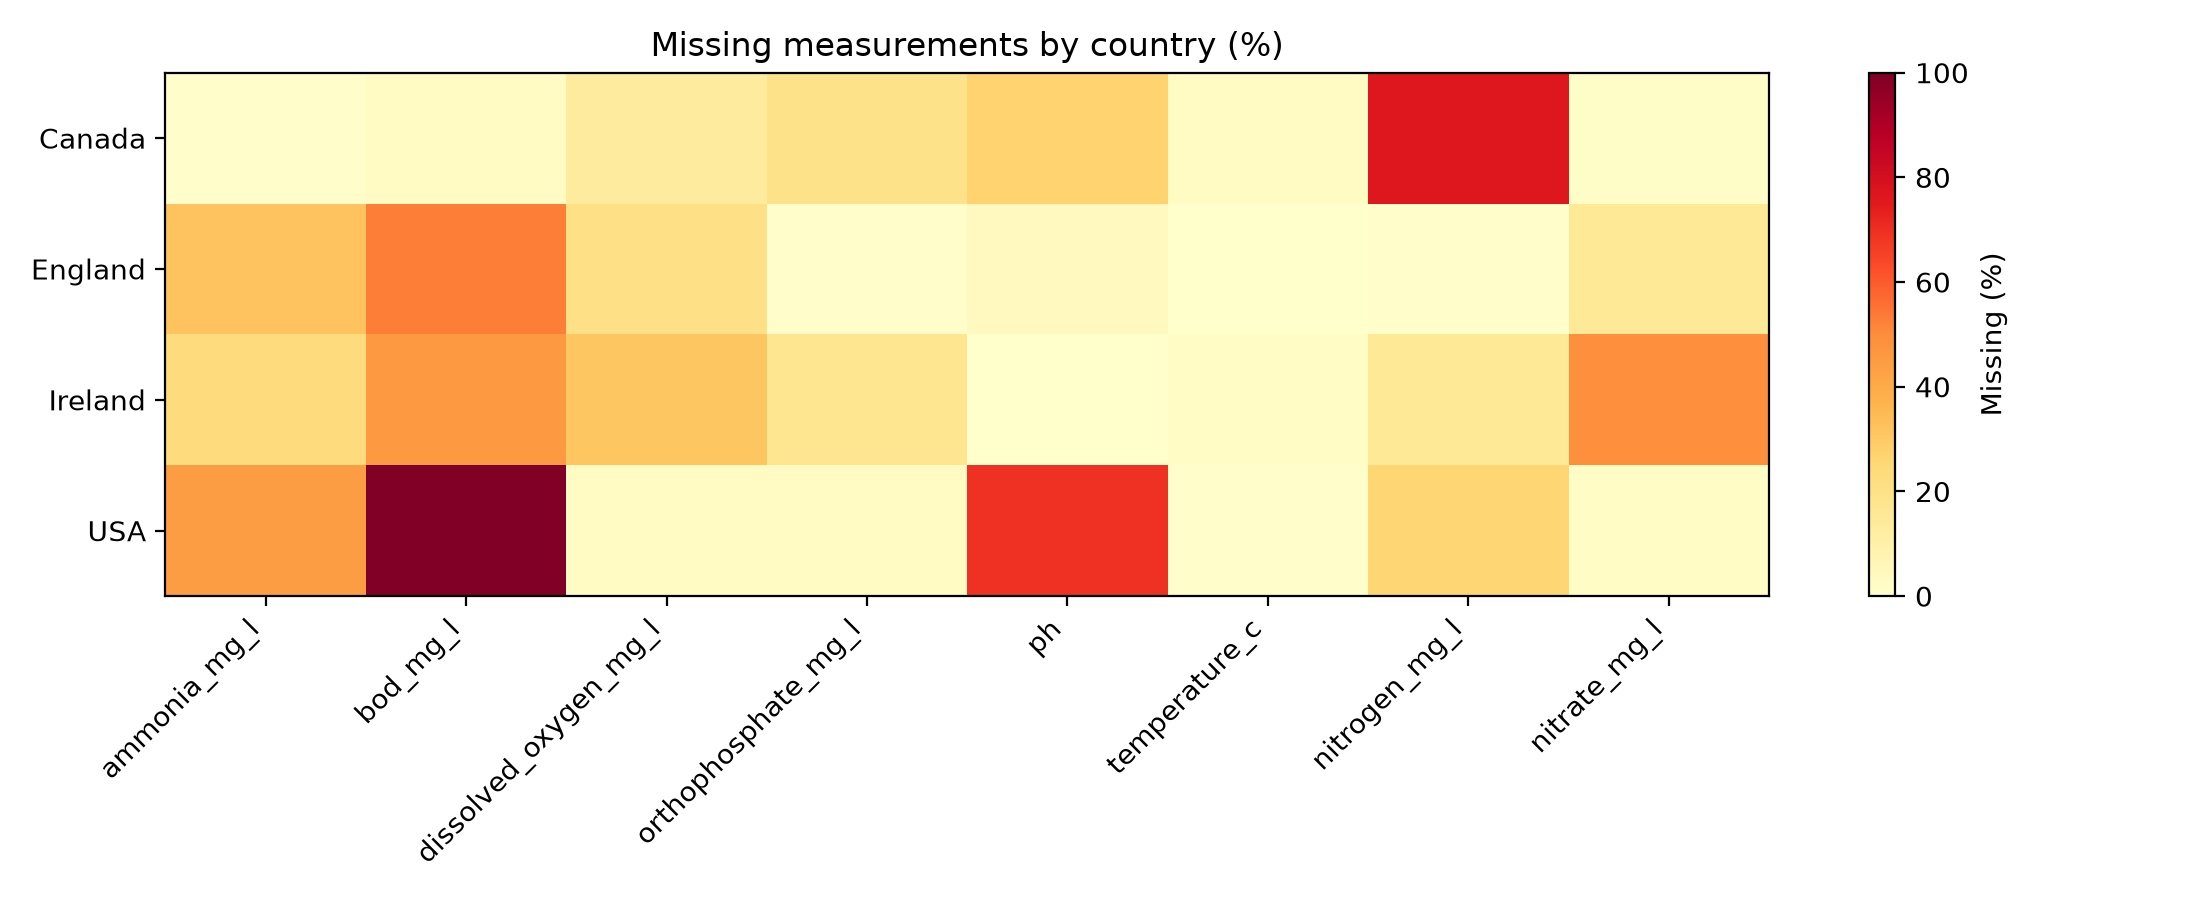
\includegraphics[width=0.8\linewidth]{../results/figures/eda_b3_missing_heatmap.png}\caption{Share of missing measurements for each country and parameter.}\label{fig:miss}\end{figure}

\subsection{The target score}
The score stops at 100, so many rows pile up there: 43.7\% of all rows are exactly 100 (Figure~\ref{fig:target}). Ireland is the most extreme with 81.6\%, England the least with 28.9\%. In terms of classes, 43.7\% of rows are Excellent, 39.9\% Good, 9.6\% Fair, 6.1\% Marginal and only 0.8\% Poor. So there is very little data on bad water, which makes it hard to predict. For this reason we also check the errors for each quality level and not only one overall score.
\begin{figure}[H]\centering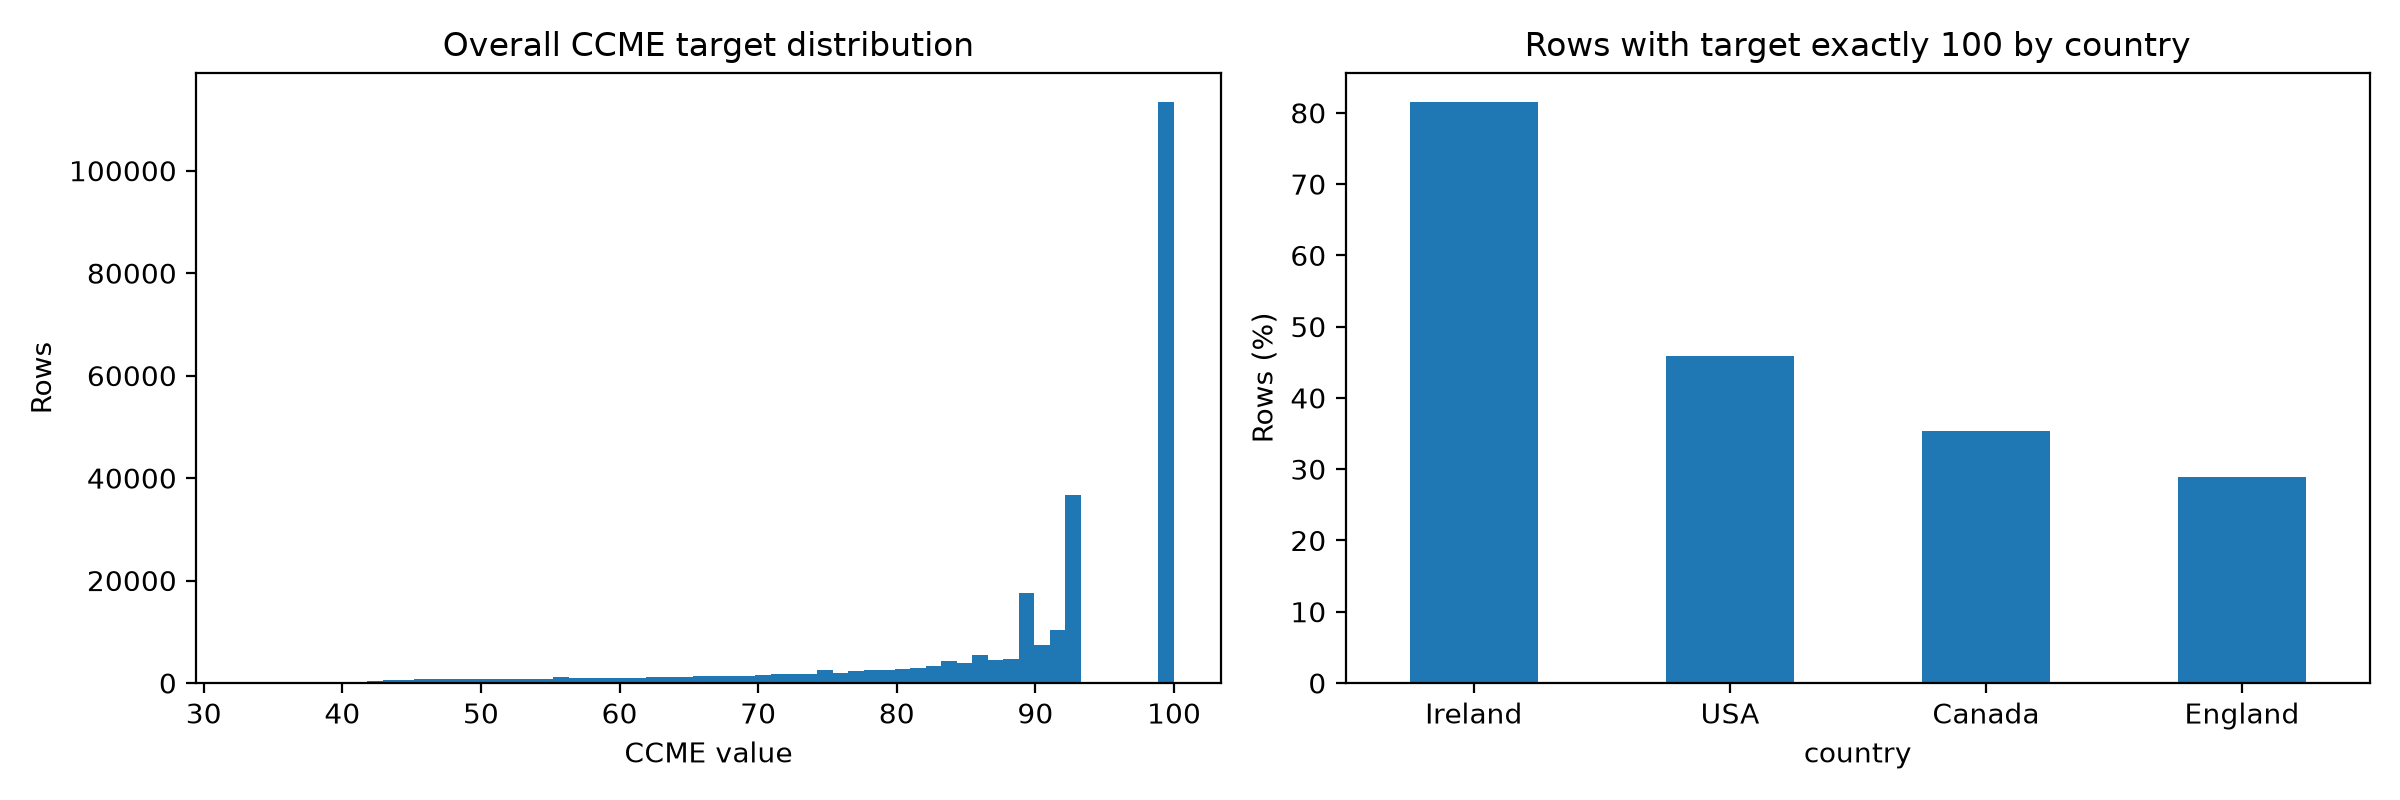
\includegraphics[width=\linewidth]{../results/figures/eda_b4_target.png}\caption{Left: distribution of the CCME score. Right: share of rows with a score of exactly 100, by country.}\label{fig:target}\end{figure}

\subsection{What drives the score}
The CCME index is calculated from eight measurements, and some of them are much more important than others (Figure~\ref{fig:corr}). We measured how strongly each one moves together with the score (Spearman correlation, where a negative value means that more of it gives a lower score). Orthophosphate is by far the strongest (-0.93), followed by ammonia (-0.54), nitrogen (-0.49), nitrate (-0.47) and BOD (-0.42). The three sensor readings are weak on their own: dissolved oxygen -0.10, pH -0.09 and temperature -0.12. If a model sees the five strong ones, it can simply recompute the formula (Section~\ref{sec:leak}), so we hide them and keep only the sensor readings. A correlation only shows that two things move together, not that one causes the other.
\begin{figure}[H]\centering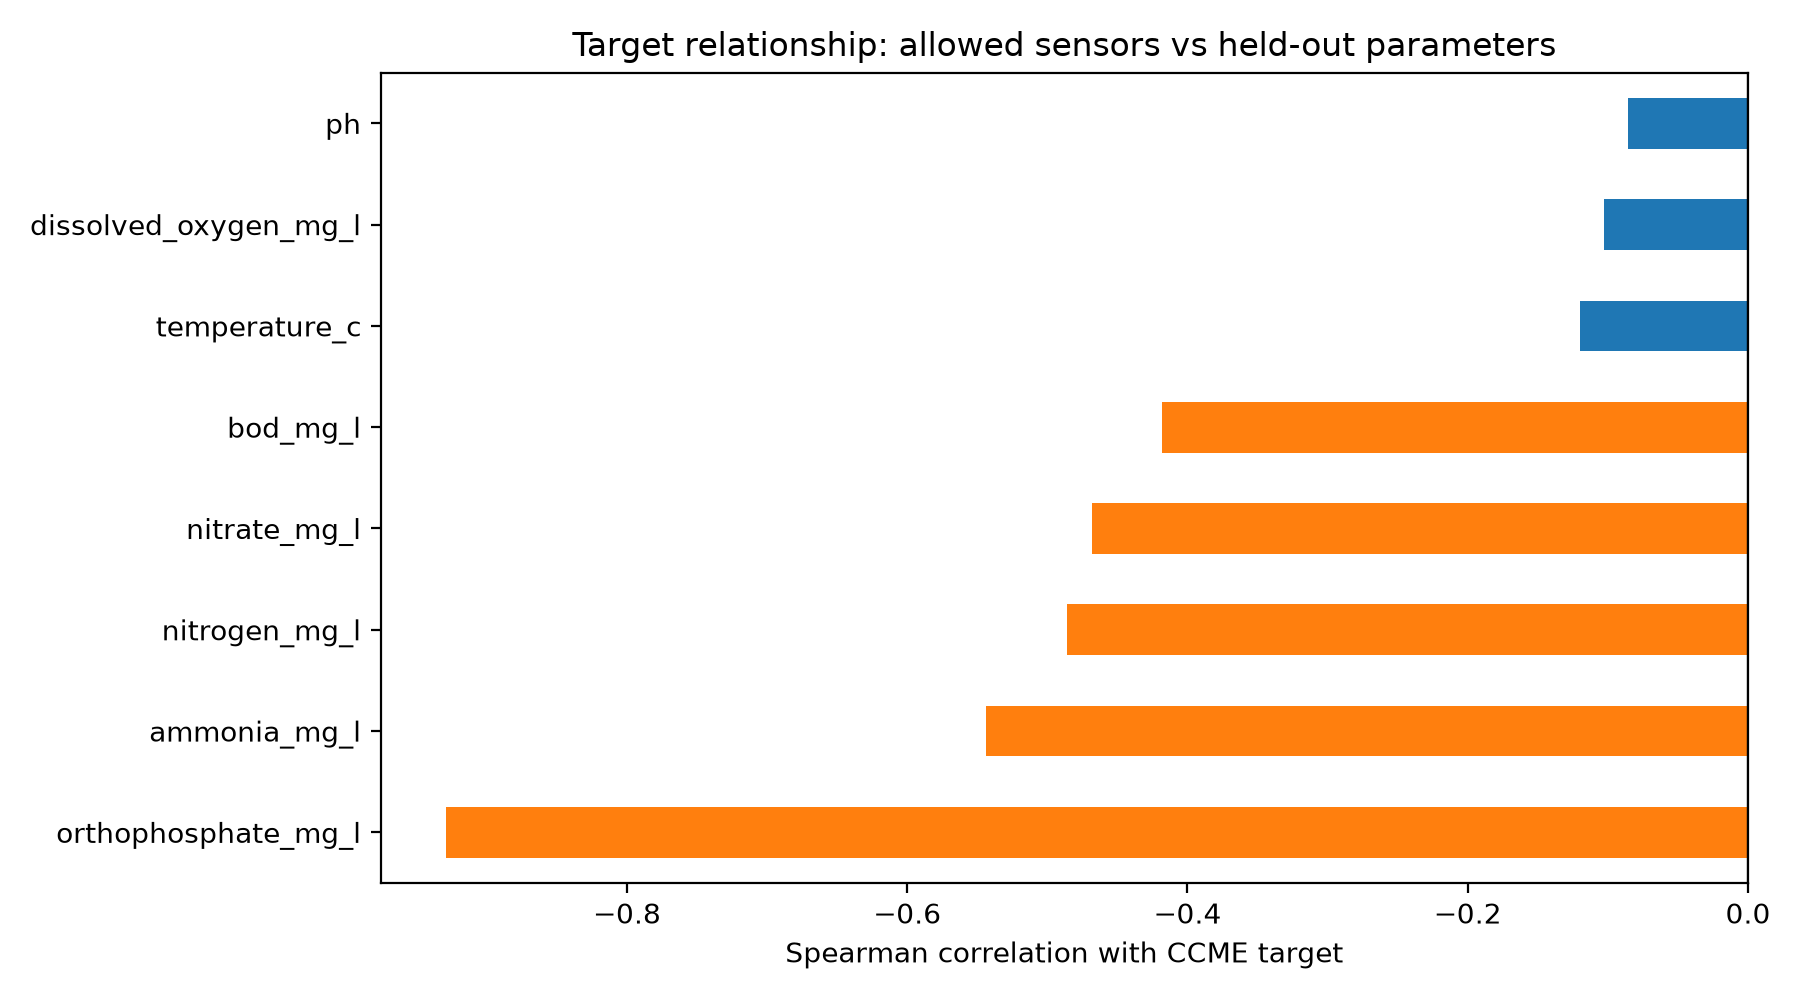
\includegraphics[width=0.7\linewidth]{../results/figures/eda_b5_corr.png}\caption{Correlation of each measurement with the score. Blue: allowed inputs. Orange: hidden from the model.}\label{fig:corr}\end{figure}

\subsection{Stations, years and seasons}
The number of rows per year is fairly steady, between about 7,000 and 14,000, with a dip in 2020 (Figure~\ref{fig:year}). Stations are very uneven: the median station has only 3 rows, 60\% of stations have 5 rows or fewer, and one station has 6,426. Rows from the same station look alike, so a random split would put the same station in both training and test data, and the model could just remember it. This is why our main split is by station. The average score also changes with the season: it is lowest in July and August (88.5) and highest in February (91.8), while dissolved oxygen drops in summer and temperature rises. This is why we turn the month into a sine and a cosine, so that December and January are next to each other.
\begin{figure}[H]\centering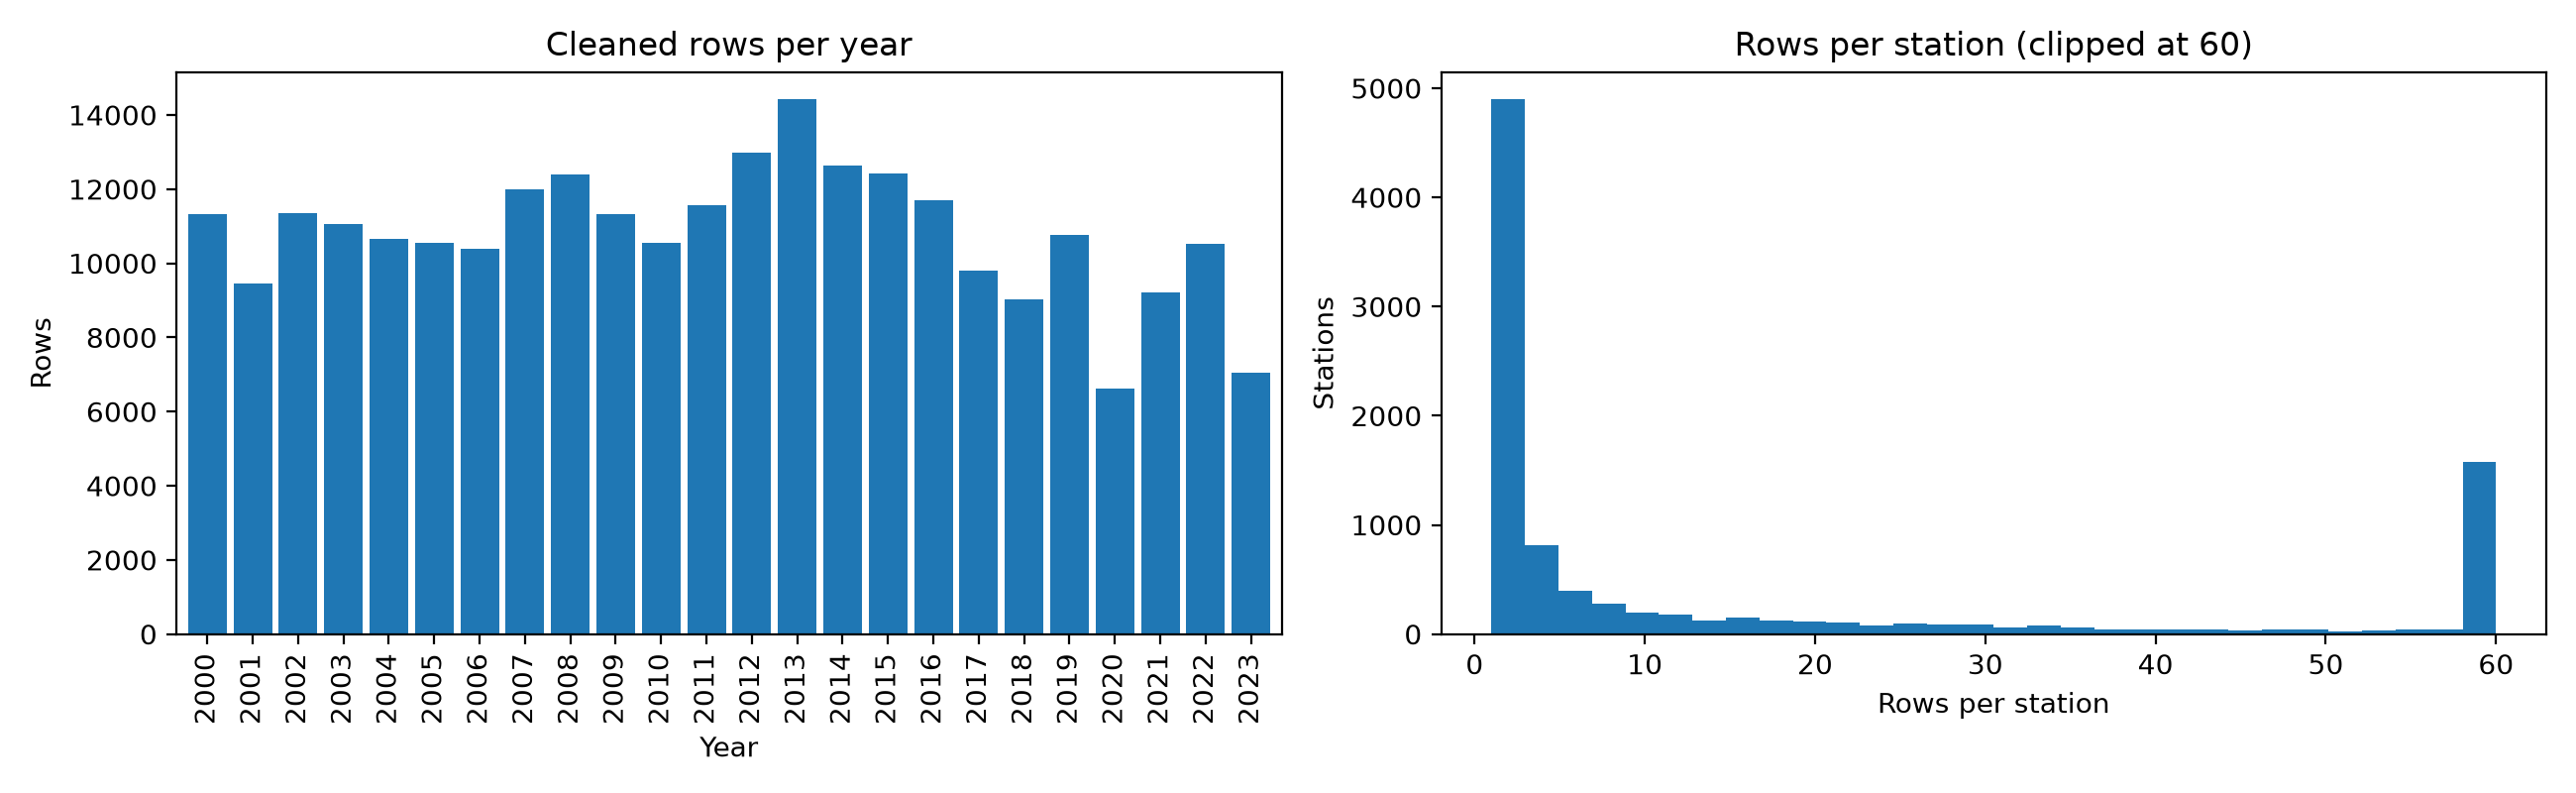
\includegraphics[width=\linewidth]{../results/figures/eda_b6_year_site.png}\caption{Left: rows per year. Right: rows per station (stations with more than 60 rows are counted as 60).}\label{fig:year}\end{figure}

\section{Methodology}
\subsection{Avoiding data leakage}\label{sec:leak}
The index is calculated from eight measurements: ammonia, BOD, dissolved oxygen, orthophosphate, pH, temperature, nitrogen and nitrate. To see how much a model can recover, we trained XGBoost on different sets of inputs and scored it on the validation data (Table~\ref{tab:leak}). With all eight measurements the score was R$^2$ = 0.991, and with our first proposed set it was 0.982. This means the model had simply learned the formula. So we removed ammonia, BOD, orthophosphate, nitrogen and nitrate from the inputs. Dissolved oxygen, pH and temperature are also part of the index, so some dependence remains, but each of them alone explains very little (R$^2$ at most 0.04).
\begin{table}[H]\caption{Validation R$^2$ of XGBoost for different input sets}\label{tab:leak}\centering\small
\begin{tabular}{p{2.5in}r}\toprule Inputs & R$^2$\\\midrule
All eight measurements & 0.991\\
First proposal (pH, temperature, ammonia, orthophosphate, nitrogen, type) & 0.982\\
Dissolved oxygen, pH, temperature only & 0.127\\
+ water type, country, month & 0.268\\
+ extra features and station history (chosen) & 0.343\\
Baseline (always the average) & $-0.005$\\\bottomrule\end{tabular}\end{table}

\subsection{Features and preprocessing}
The models use 14 inputs: dissolved oxygen, pH, temperature, the month (as a sine and a cosine, so that December is next to January), oxygen saturation, dissolved oxygen $\times$ temperature, the station's average past dissolved oxygen, pH and temperature, the number of earlier samples at the station, days since the previous sample, water body type and country. The past averages only use earlier sampling dates of the same station, so nothing from the future is used. Missing values are filled with the median of the training data (and a ``was missing'' flag is added), categories are one-hot encoded, and values are scaled for Ridge only. All of this is learned from the training data only.

\subsection{Train, validation and test split}
Our main split is by station. All rows of a station go to only one part: 70\% of rows for training, 10\% for validation and 20\% for testing (181,747 / 26,054 / 51,973 rows from 6,583 / 1,136 / 2,221 stations). This way the test shows how a model does at a place it has never seen. A random split of rows would put the same station in both parts, and the model could do well just by remembering the station. Our second split is by year: training up to 2015, validation 2016--2017 and test 2018 onwards. It checks how the models do on later data. We choose settings using the validation data only, and use the test data once at the end.

\subsection{Models and tuning}
The baseline always predicts the average of the training data. Ridge Regression is a straight-line model with a penalty that keeps the numbers small. Random Forest averages the answers of many deep decision trees, which makes it more stable. XGBoost builds trees one after another, where each new tree tries to fix the mistakes of the earlier ones. We tuned each model on the validation data by trying a small grid of settings, changing one setting at a time: Ridge penalty $\alpha$ from $10^{-3}$ to $10^{3}$; Random Forest depth 6--16 and minimum leaf size 2--20 (300 trees); XGBoost depth 4--10, learning rate 0.03--0.1 and 300 or 600 trees. The settings with the lowest validation RMSE were chosen: Ridge $\alpha=0.001$; Random Forest depth 16 and minimum leaf size 5; XGBoost depth 8, learning rate 0.03, 300 trees, row sampling 0.8, feature sampling 0.8 and L2 weight 1.0. The random seed was 42.

\subsection{Metrics and confidence intervals}
\begin{equation}\mathrm{MAE}=\frac{1}{n}\sum_{i=1}^{n}|y_i-\hat{y}_i|,\end{equation}
\begin{equation}\mathrm{RMSE}=\sqrt{\frac{1}{n}\sum_{i=1}^{n}(y_i-\hat{y}_i)^2},\end{equation}
\begin{equation}R^2=1-\frac{\sum_i(y_i-\hat{y}_i)^2}{\sum_i(y_i-\bar{y})^2}.\end{equation}
MAE is the average size of the error, and RMSE is similar but gives more weight to big errors. For both, lower is better. R$^2$ tells us how much better the model is than always guessing the average: 1 is perfect and 0 is no better than the average. A test set is only one sample of stations, so a score has some luck in it. To measure this, we repeated the evaluation 2,000 times on stations drawn again at random (keeping all rows of a station together, because the rows of one station are similar) and used the middle 95\% of the results as the 95\% confidence interval. To compare two models fairly, we used the same re-drawn stations for both and looked at the difference between their errors.

\section{Results}
\subsection{Validation results}
On the validation data XGBoost was best (MAE 7.729, RMSE 11.205, R$^2$ = 0.348), just ahead of Random Forest (7.773, 11.247, 0.343). Ridge reached R$^2$ = 0.219 and the baseline $-0.005$. On the training data, Random Forest scored R$^2$ = 0.558 and XGBoost 0.461, so Random Forest fits the training data more closely and overfits more. Ridge scored about the same on training data (0.211), because it is too simple to learn much.

\subsection{Test on unseen stations}
Table~\ref{tab:test} shows the final test results from \texttt{results/final\_results.csv}.
\begin{table}[H]\caption{Test results on unseen stations, with 95\% confidence intervals for R$^2$}\label{tab:test}\centering\footnotesize
\begin{tabular}{@{}lrrrl@{}}\toprule Model & MAE & RMSE & R$^2$ & 95\% CI\\\midrule
Baseline (average) & 9.570 & 13.159 & -0.001 & [-0.009, 0.000]\\
Ridge & 8.329 & 11.733 & 0.205 & [0.174, 0.233]\\
Random Forest & 7.598 & 11.179 & 0.278 & [0.230, 0.324]\\
XGBoost & 7.543 & 11.058 & 0.293 & [0.246, 0.340]\\\bottomrule\end{tabular}\end{table}
XGBoost is the best model. The confidence intervals of XGBoost and Random Forest overlap, but both models are affected by the same lucky or unlucky stations. So we compared them on the same re-drawn stations: XGBoost's RMSE was lower by 0.121 (95\% interval $-0.186$ to $-0.059$). This means XGBoost is better in a consistent way, but only by a small amount. Both tree models are clearly better than Ridge (XGBoost's RMSE is 0.674 lower) and than the baseline (2.101 lower). Still, R$^2$ below 0.30 means that most of the variation in the score is not explained. The test R$^2$ is lower than the validation R$^2$ (0.293 against 0.348 for XGBoost). One reason is that we picked the settings that looked best on the validation data. Another is probably that the test stations are different and harder. We did not separate these two reasons.

\subsection{Test on later years}
Results for 2018 onwards: baseline MAE 9.101, RMSE 10.693, R$^2$ = $-0.338$; Ridge MAE 6.738, RMSE 8.786, R$^2$ = 0.097; Random Forest MAE 5.596, RMSE 8.310, R$^2$ = 0.192; XGBoost MAE 5.449, RMSE 8.047, R$^2$ = 0.243. For this test the models were trained again on the year split, with the same settings. These numbers should not be mixed with the station test, because the test data are different. For example, the baseline gets a negative R$^2$ here, which shows that the scores changed after 2015. The order of the models stays the same: XGBoost, Random Forest, Ridge, baseline.

\subsection{Where do the models go wrong?}
The overall score hides big differences between countries (Table~\ref{tab:country}). England makes up 70\% of the test rows, and the model helps least there (its MAE is only 6\% lower than the baseline's). Ireland shows the biggest improvement, but 82\% of Irish samples are exactly 100, so there is little left to explain and its R$^2$ is close to zero. The USA and Canada have few rows, so their results are not very reliable.
\begin{table}[H]\caption{XGBoost test results by country}\label{tab:country}\centering\small
\begin{tabular}{lrrrr}\toprule Country & Rows & MAE & Baseline MAE & R$^2$\\\midrule
England & 36,396 & 9.25 & 9.86 & 0.194\\
Ireland & 14,443 & 3.30 & 8.91 & 0.026\\
USA & 580 & 5.88 & 9.35 & 0.156\\
Canada & 554 & 7.63 & 8.15 & 0.080\\\bottomrule\end{tabular}\end{table}

The error also depends on how good the water really is (Table~\ref{tab:band}). When the true score is below 60 (poor water), the model guesses about 31 points too high on average, and for perfect water (100) it guesses about 5.5 points too low. So the guesses are pulled towards the middle. This happens because the five main measurements are hidden, so the model cannot tell when water is really bad, and 44\% of all samples are exactly 100, so a ``fairly good'' guess is usually safe. Several of the hardest stations are poor-quality places near sewage works or industrial discharges that the model predicts as good.
\begin{table}[H]\caption{XGBoost test error by true quality level}\label{tab:band}\centering\small
\begin{tabular}{lrrr}\toprule True score & Rows & MAE & Mean error\\\midrule
below 60 & 2,719 & 30.98 & $+30.98$\\
60 to 80 & 6,032 & 12.52 & $+12.15$\\
80 to 95 & 20,502 & 5.19 & $-1.90$\\
100 & 22,720 & 5.54 & $-5.52$\\\bottomrule\end{tabular}\end{table}

\subsection{Which inputs matter?}
To see how much the models depend on some inputs, we trained XGBoost again with them removed and checked the validation score. With all inputs, R$^2$ was 0.348. Without country it dropped to 0.274, without the station history to 0.271, and without both to 0.162. SHAP gives the same picture on 3,000 test rows: country is the most important input (average effect 4.75 points), followed by the station's past dissolved oxygen (1.40), temperature (1.32) and the station's past pH (1.19). So a good part of the score comes from knowing which country and station a sample is from. This may not work well in a new region. SHAP shows what the model uses, not what causes the water quality.

\begin{figure}[H]\centering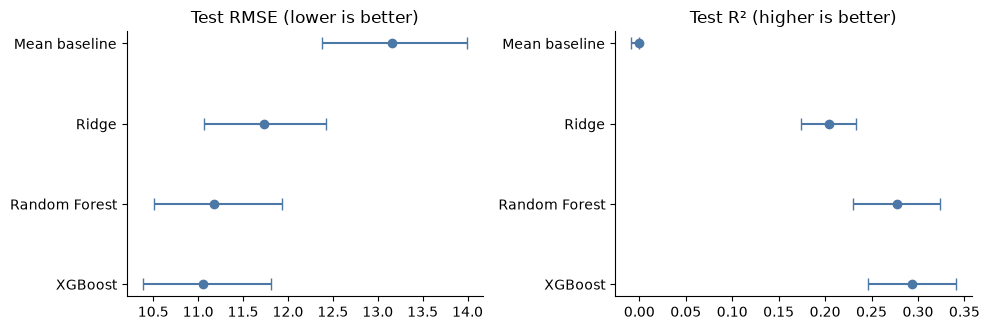
\includegraphics[width=0.85\linewidth]{../results/figures/eval_ci.png}\caption{Confidence intervals of the test scores.}\label{fig:ci}\end{figure}
\begin{figure}[H]\centering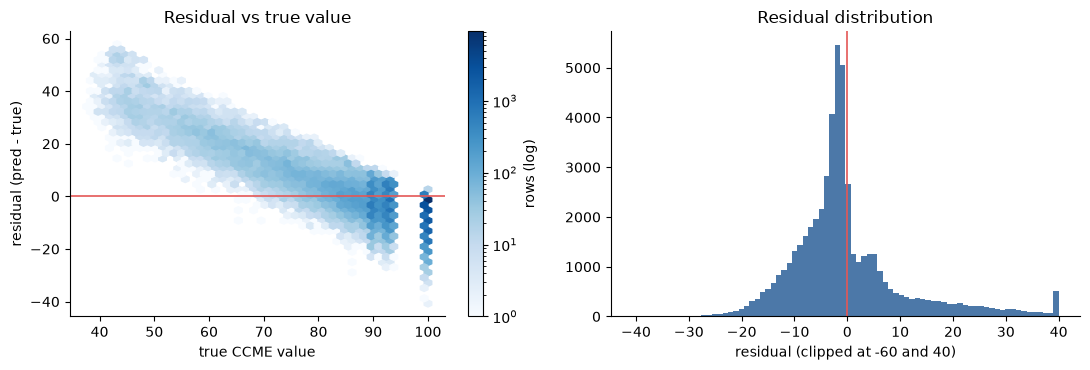
\includegraphics[width=0.85\linewidth]{../results/figures/eval_residuals.png}\caption{Errors of the test predictions.}\label{fig:resid}\end{figure}
\begin{figure}[H]\centering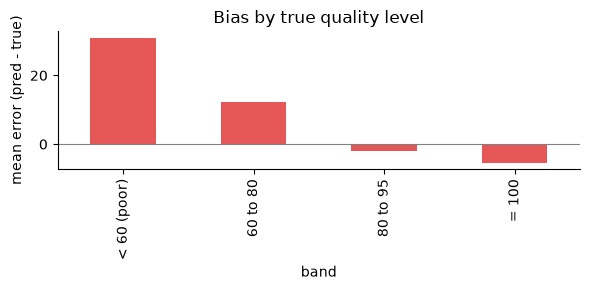
\includegraphics[width=0.85\linewidth]{../results/figures/eval_bias_by_band.png}\caption{Average error of XGBoost by true water quality level.}\label{fig:band}\end{figure}
\begin{figure}[H]\centering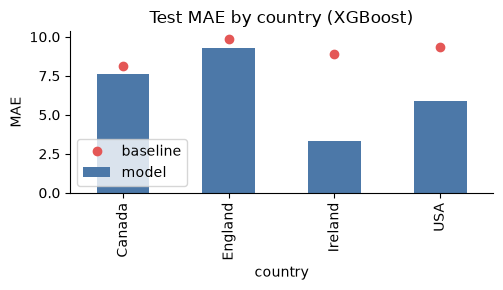
\includegraphics[width=0.85\linewidth]{../results/figures/eval_by_country.png}\caption{XGBoost test performance by country.}\label{fig:country}\end{figure}
\begin{figure}[H]\centering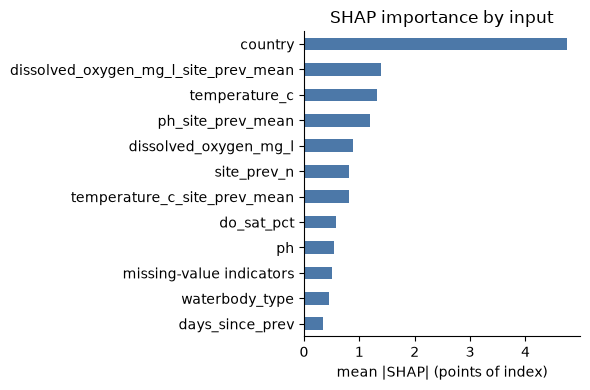
\includegraphics[width=0.85\linewidth]{../results/figures/eval_shap_grouped.png}\caption{Importance of each input for XGBoost (SHAP).}\label{fig:shap}\end{figure}

\section{Discussion}
The tree models work better than the baseline and Ridge, even with the reduced set of inputs. XGBoost is best on both test types, and Random Forest is close; the comparison on the same re-drawn stations shows that XGBoost's lead is real but small. On later years the errors are lower but R$^2$ is also lower than on new stations. This is because the data are different, so we do not treat it as one split being better than the other. Many samples sit at 100, so one measure alone does not tell the whole story, and we report MAE, RMSE and R$^2$ together with results by country and by quality level. The biggest weakness is that polluted water is predicted as better than it is, which is the more harmful mistake in real monitoring.

\section{Limitations and Future Work}
The model cannot replace laboratory tests or official checks. Countries and monitoring practices differ, and the filled-in values in the source data may affect the score. The test R$^2$ is moderate, which is expected because the five main measurements are hidden on purpose. We chose settings using one validation split and did not use cross-validation, so the validation scores are somewhat optimistic. The best Random Forest depth and the best XGBoost learning rate were at the edge of what we tried, so slightly better settings may exist. England has most of the data, while the USA and Canada have very little. In Phase 2 we plan to train a small neural network (MLP) on the same inputs and the same splits, and compare it fairly without touching the test set while choosing the model. We also want to check how the models work on stations from regions with little data.

\section{Conclusion}
We compared an average-only baseline, Ridge Regression, Random Forest and XGBoost for predicting the CCME water quality index without using the measurements it is calculated from. On unseen stations XGBoost gave MAE 7.543, RMSE 11.058 and R$^2$ = 0.293, slightly but consistently better than Random Forest. On later years it gave MAE 5.449, RMSE 8.047 and R$^2$ = 0.243. Tree models are good starting points, but they do not predict the index very accurately: they over-estimate poor water, and much of their skill comes from the country and the station history. The next step is a fair comparison with a neural network.

\bibliographystyle{plain}\bibliography{references}
\end{document}
